\documentclass[10pt,conference,compsocconf]{IEEEtran}

\usepackage[dvipsnames]{xcolor}
\usepackage[colorlinks = true,
            linkcolor = black,
            urlcolor  = BlueViolet,
            citecolor = blue,
            anchorcolor = blue]{hyperref}
\usepackage{graphicx}	% For figure environment
\usepackage[english]{babel}
\usepackage{gensymb}
\usepackage{amsmath}
\usepackage{cases}


\begin{document}
\title{Classification of H$^0$ decaying from noise: comparing machine learning methods.}

\author{
 \textit{Authors:} \href{mailto:gaia.carparelli@epfl.ch}{Gaia Carparelli}, \href{mailto:hugues.vinzant@epfl.ch}{Hugues Vinzant}, \href{mailto:axel.bisi@epfl.ch}{Axel Bisi}  \\
 Project 1 in \textit{CS-433 Machine Learning}, Ecole Polytechnique F\'{e}d\'{e}rale de Lausanne, Switzerland
}

\maketitle

\begin{abstract}
This first machine learning project joins an online competition: distinguishing the Higgs boson (H$^0$) from noise with original data from CERN. Several machine learning functions were implemented using the Python \verb|numpy| library in order to explore features, to train and test different classification models and to find the most accurate one. The final, cross-validated, model was based on the division of the data set into three subsets based on the number of jets using ridge regression to train each subset individually; the final score was 0.8286 on the online platform Kaggle.
\end{abstract}

%-----Introduction-----
\section{Introduction}

Following the discovery of the Higgs boson, fundamental for a more complete understanding of subatomic particles and forces in nuclear physics, experiments were run to understand its decay, which produces specific particles as a signature. As such, the aim of the Higgs boson machine learning challenge is to predict whether a measured signal corresponds to the Higgs boson or to background noise. In this binary classification project, basic regression methods were compared, preceded by feature analysis and pre-processing of the data provided by the competition. A k-fold cross-validation was implemented to identify the best parameters as well as to have an unbiased estimate of the classification model's performance.

%-----Models and Methods-----
\section{Models and Methods}
\label{sec:methods}
The given data set consisted in hundred of thousands of samples and 30 features such as particle mass, momentum and derivatives. To achieve a satisfying binary classification, features were engineered, classification models were implemented using the training set and evaluated using the testing set.

\subsection{Data exploration and feature processing}
Observing the class-differentiated distributions of features did not provide much insight of possibly discriminant features. 
Yet, feature \#22 (\verb|PRI\_jet\_num|) was composed of categorical integers from 0 to 3, leading to the idea of dividing the data set into three subsets, corresponding to '0 jet', '1 jet', '2 or more jets' respectively for each integer. 
The third subset combines samples with both integers 2 and 3 of feature \#22 as they have the same number of relevant features with non-null variance.
Indeed, variance was checked for each feature per subset and non-relevant features with null variance were removed under the basis that they are uninformative since they do not allow for any sample discrimination.
Thus, the number of relevant features with non-null variance differs for each subset. Consequently, each subset has its own model which is optimized individually.
Thus, the resulting subsets $\mathbf{X}_{i, i=0,1,2}$ have unique dimensions as described in Table \ref{tab:subset}. The resulting data set structure is depicted in Fig.\ref{data}.

%Figure 2:Data structure
\begin{figure}
\begin{center}
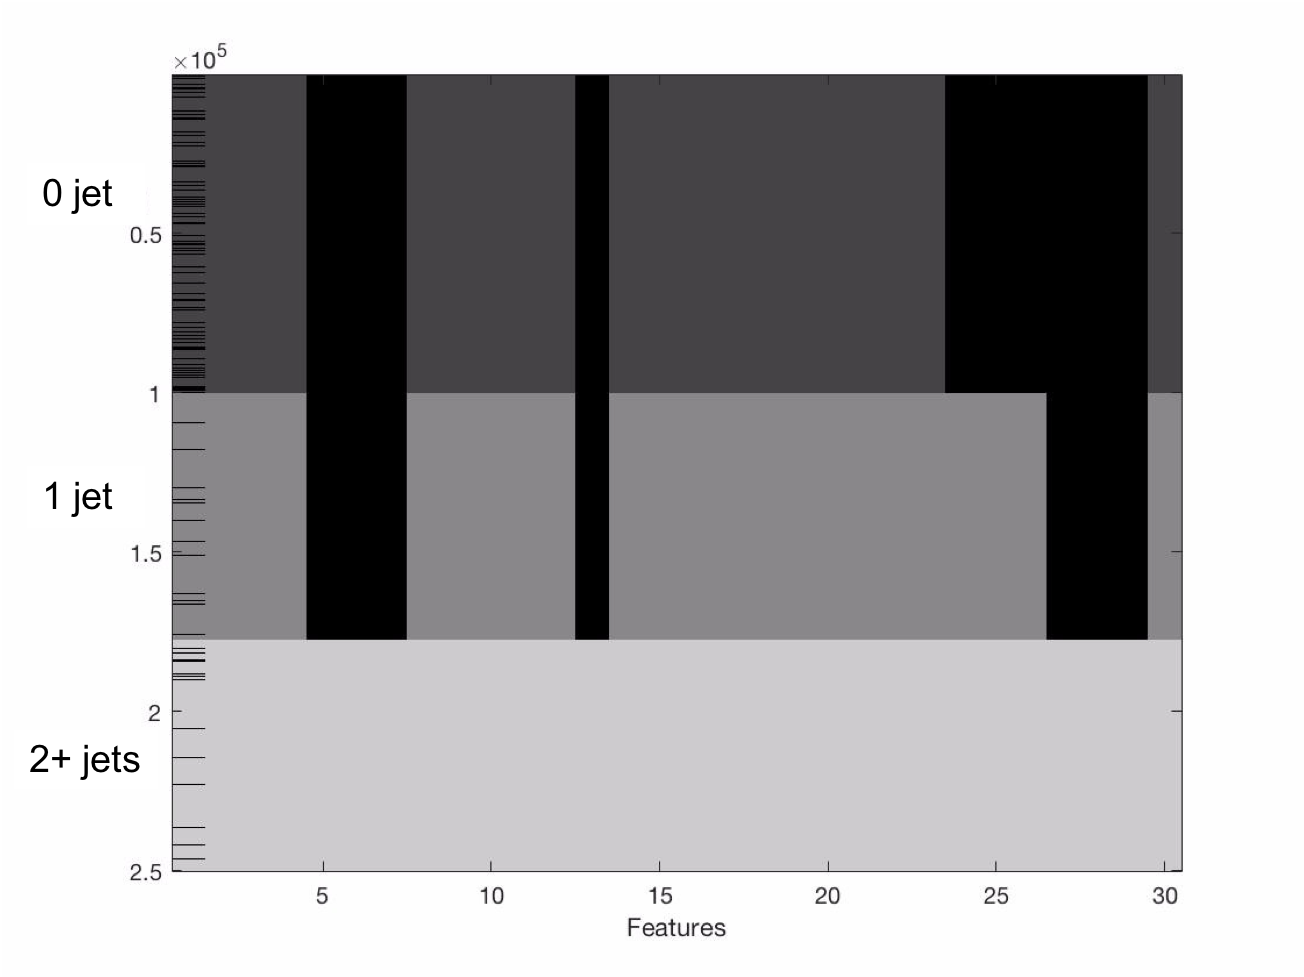
\includegraphics[scale=0.22]{data.png}
\caption{Data structure per subset: black areas correspond to removed features except column 0.}
\label{data}
\end{center}
\end{figure}


%Table 1 : Subset dimensions
\begin{table}[]
    \centering
     \caption{Train subset dimensions after feature selection.}
    \label{tab:subset}
    \begin{tabular}{|c|c|c|c|}
    \hline
    \textbf{Subset} $i$ &  '0 jet' &  '1 jet' & '2+ jets' \\
    \hline
    \textbf{Size} & (99913, 18) & (77544, 22) & (72543, 30) \\
    \hline
     \end{tabular}
\end{table}

One of the first issue encountered was dealing with meaningless values; jet division combined with variance-based selection allowed to get rid of all meaningless values except from the ones in column 0.
For feature 0, missing values were either estimated using least squares regression or set to zero which makes sense theoretically as undefined values were caused by some signal acquisition specificity e.g. topology of the event too far from the expected one \cite{info}.
%For each subset $i$ with $d_i$ features, optimal weights $\mathbf{w}^{\star}_i$ were found as followed:

%\begin{equation}
 %   \mathbf{w}^{\star}_i = %(\mathbf{X}^{\top}_{:d_i}\mathbf{X}_{:d_i})^{-1}\mathbf{X}^{\top}_{:d_i}\m%athbf{y}
%\end{equation}

%while the resulting --999 values of feature \#0 were imputed, per subset:

%\begin{equation}
 %   \mathbf{\hat{y_i}} = \mathbf{X}^{\top}_{:0,i}\mathbf{w}^{\star}_i,
%\end{equation}
%where $\mathbf{X}^{\top}_{:0,i}$ corresponds to the first feature column of %the the data matrix for subset $i$.

Therefore, subsets could be standardized feature-wise to zero-mean and unit standard deviation in order to adjust for any dissimilar ranges of values that could be observed between features. Standardization enables pre-conditioning of the optimization problem through which an adequate step-size may be found for gradient descent.
Of course the test set was standardized based on mean and standard deviation of the train set.

In addition, the number of samples was large enough to perform augmentation of the remaining selected features using polynomial expansion of degree $n$. The resulting model for sample $y_i$ is then:
\begin{equation}
y_i = a_0 + a_1x + a_2x^2 + ... + a_nx^n + \epsilon, i = 1, ... ,N,
\end{equation}
where $a_0$ represents the offset, a vector of ones.

\subsection{Models and cross-validation}

For the final model, ridge regression, also with and without estimation of column 0 (models A \& B) was used and compared with regularized logistic regression with and without estimation of column 0 (models C \& D). Only these two regression methods from the six methods implemented were compared for several reasons.
First, gradient descent and stochastic gradient descent were not used because convergence to global optimum is not guaranteed, are time-inefficient (no explicit solutions for the weights but iterative computations) unlike least squares with normal equations.
Then, ridge regression and regularized logistic regression were respectively preferred over least squares and basic logistic regression because less sensitive to over-fitting due to the penalizing regularization factor $\lambda$.

Chosen models were compared using $10$-fold cross-validation where model parameters, such as degree $n$ and $\lambda$, were chosen as to maximize the prediction score in an unbiased manner. For the final model, ridge regression was used to estimate optimal weights $\mathbf{w}^{\star}_{ridge}$:

\begin{equation}
    \mathbf{w}^{\star}_{ridge} = (\mathbf{X}^{\top}\mathbf{X} + \lambda'\mathbf{I})^{-1}\mathbf{X}^{\top}\mathbf{y},
\end{equation}
where  $\lambda' = 2N\lambda$. Classification of samples, $\mathbf{\hat{y}}'$, in 'signal' (1) and 'background' (-1) is based on the computed label prediction $\mathbf{\hat{y}}$, as follows:

\begin{equation} \label{eq:3}
\mathbf{\hat{y}}' =  
\begin{cases}
1, &\mbox{if } \mathbf{\hat{y}} \ge 0 \\
-1,  & \mbox{if } \mathbf{\hat{y}} < 0 \\
\end{cases}
\end{equation}

The predictions $\mathbf{\hat{y}}'$ were then reconstructed into one unique prediction vector $\mathbf{\hat{Y}}$ assembled from the three subset predictions. Finally, evaluation of the validated model was performed using Kaggle's online platform.

%-----Results-----
\section{Results} 
\label{sec:results}
After subset division and computing of feature variance, it appeared that, as described in Table \ref{tab:subset}, 18, 22 and 30 features were relevant to build models respectively in 0, 1 and 2 or more jets.
As illustrated in Table \ref{tab:scores} the four implemented models gave different results. First, on each subset, ridge regression gave higher scores than regularized logistic regression. Further analysis showed that least squares estimation of the meaningless values of column 0 did not improve the accuracy of the model, contrariwise the best scores were obtained on the training data where meaningless entries of column 0 were set to zero before standardization.
In conclusion, the final and best model was model B (ridge regression without estimation of feature 0).

Cross validation determined best parameters for model B, as in Table \ref{tab:param}.  Fig. \ref{param} illustrates how the model accuracy evolves depending on both the chosen degree $n$ and $\lambda$. Finally, the optimal $\lambda$ was the same for the three subsets (1e-4) while the degree $n$ was slightly higher in the '2 or more jets' subset.
Using these parameters, the final score obtained on Kaggle was 82.859\%.

%Figure 1: Best parameters
\begin{figure}
\begin{center}
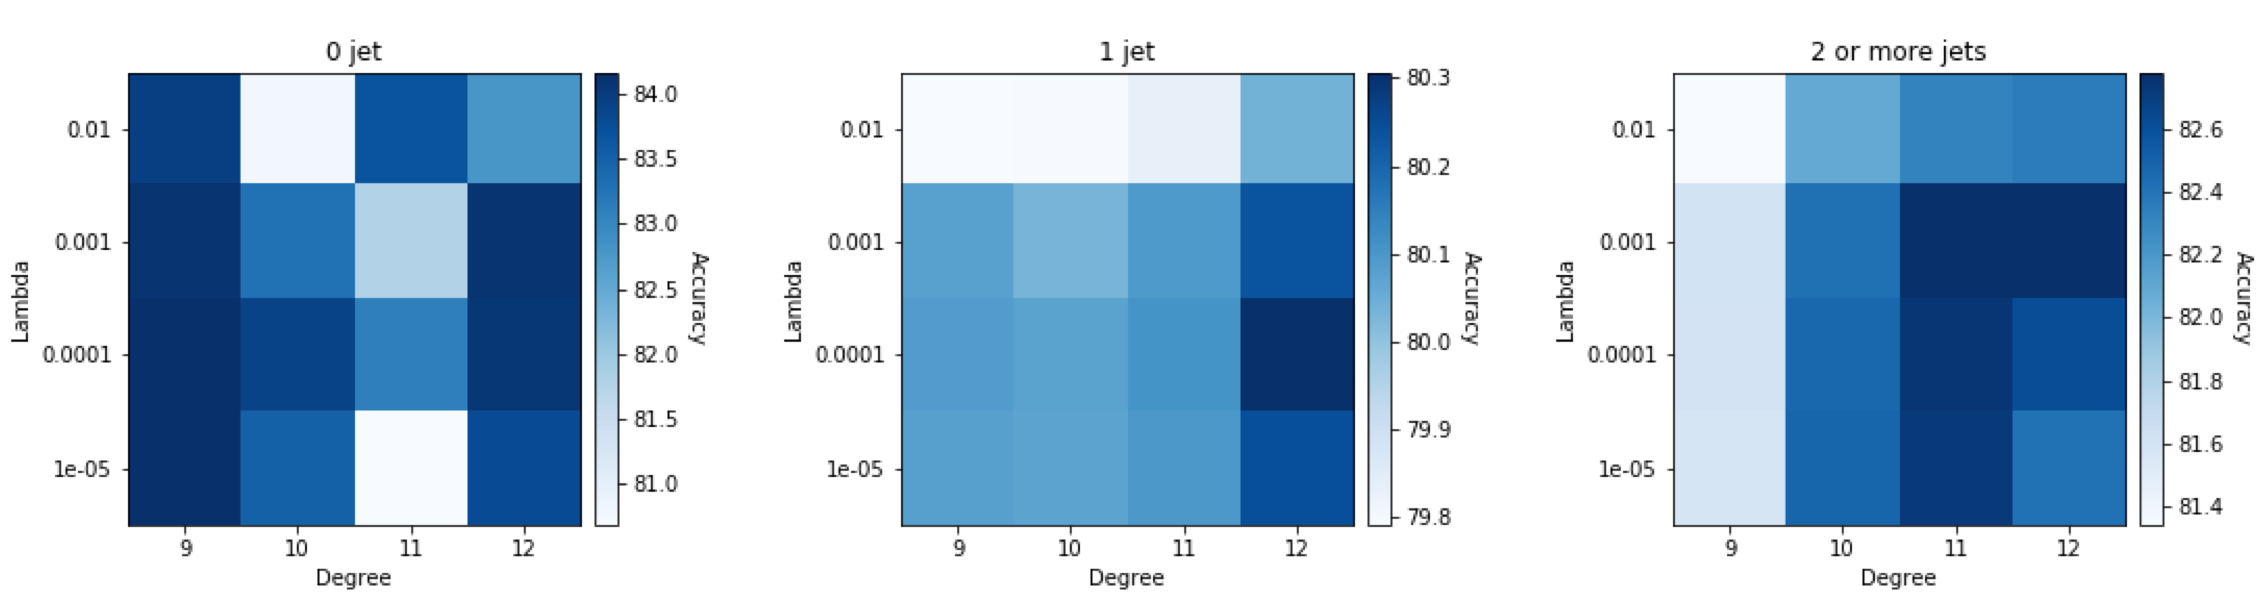
\includegraphics[scale=0.235]{best_parameters.png}
\caption{Hyperparameter optimization for model A: left to right, figures correspond to sets '0 jet', '1 jet' and '2+ jets' with the left $y$-axis, $x$-axis and right $y$-axis respectively the penalty tuner $\lambda$, the extension degree $n$ and the prediction score.}
\label{param}
\end{center}
\end{figure}

%Table 3: Performance score per model
\begin{table}[]
    \centering
    \caption{Prediction scores for each sub-set and model.}
    \label{tab:scores}
    \begin{tabular}{|c|c|c|c|c|}
    \hline
    \textbf{Model} &  '0 jet' &  '1 jet'  & '2+ jets' & 'Kaggle'\\
    \hline
    \textbf{A} & 0.84171 & 0.80306 & 0.82781 & 0.82647\\
    \hline
    \textbf{B} & 0.84242 & 0.80562 & 0.83335 & 0.82859\\
    \hline
     \textbf{C} & 0.82374 & 0.75944 & 0.76174 & 0.78088\\
    \hline
     \textbf{D} & 0.82362 & 0.75889 & 0.76322 & 0.79523
 \\
    \hline
    \end{tabular}
    \vfill
\end{table}

%Table 3: Hyperparameters optimization 
\begin{table}[h!]
    \centering
    \caption{Optimized hyper-parameters for model B.}
    \label{tab:param}
    \begin{tabular}{|c|c|c|c|}
    \hline
     \textbf{Parameter} &  '0 jet' &  '1 jet' & '2+ jets'  \\
    \hline
    Degree $n$ & 12 & 12 & 13 \\
    \hline
     \textit{$\lambda$} & 1e-4 & 1e-4 & 1e-4  \\
    \hline
     \end{tabular}
     \vfill
\end{table}

%-----Discussion-----
\section{Discussion}
\label{sec:discussion}
Although ridge regression gave rather satisfying results, it is important to notice that this is not a real binary classifier and it only could have been applied to our problem thanks to the threshold function (\ref{eq:3}) discussed above. Knowing that, regularized logistic regression which uses probability to predict the final label is more suitable for classification problems yet its computational time is longer than for ridge regression. Also, the regularized logistic regression algorithm is more complex, especially for large data sets, and was implemented it too late to be able to push its optimization as far as desired.

Despite the high number of samples and, as a rule of thumb, 100 samples per feature are needed at least, one way to improve our model would be to explore the nature of features. Correlation between features could be analyzed, to perhaps combine highly correlated ones. Some additional physics background for feature understanding would have been helpful to see which features carry little information and which are statistically important for the classification model.

Also delving deeper into feature engineering, e.g. alternate feature augmentation with logarithmic, square-roots, sinusoidal or Gaussian bases would have potentially allowed insightful comparison.

%\section*{Acknowledgements}
\begin{thebibliography}{}
\bibitem{info}
C.~Adam-Bourdarios, G.~Cowan, C.~Germain, I.~Guyon, B.~K\'{e}?l, D. ~ Rousseau.
Learning to discover: the Higgs boson machine learning challenge, 2014.
\end{thebibliography}


\end{document}